\documentclass[1p]{elsarticle_modified}
%\bibliographystyle{elsarticle-num}

%\usepackage[colorlinks]{hyperref}
%\usepackage{abbrmath_seonhwa} %\Abb, \Ascr, \Acal ,\Abf, \Afrak
\usepackage{amsfonts}
\usepackage{amssymb}
\usepackage{amsmath}
\usepackage{amsthm}
\usepackage{scalefnt}
\usepackage{amsbsy}
\usepackage{kotex}
\usepackage{caption}
\usepackage{subfig}
\usepackage{color}
\usepackage{graphicx}
\usepackage{xcolor} %% white, black, red, green, blue, cyan, magenta, yellow
\usepackage{float}
\usepackage{setspace}
\usepackage{hyperref}

\usepackage{tikz}
\usetikzlibrary{arrows}

\usepackage{multirow}
\usepackage{array} % fixed length table
\usepackage{hhline}

%%%%%%%%%%%%%%%%%%%%%
\makeatletter
\renewcommand*\env@matrix[1][\arraystretch]{%
	\edef\arraystretch{#1}%
	\hskip -\arraycolsep
	\let\@ifnextchar\new@ifnextchar
	\array{*\c@MaxMatrixCols c}}
\makeatother %https://tex.stackexchange.com/questions/14071/how-can-i-increase-the-line-spacing-in-a-matrix
%%%%%%%%%%%%%%%

\usepackage[normalem]{ulem}

\newcommand{\msout}[1]{\ifmmode\text{\sout{\ensuremath{#1}}}\else\sout{#1}\fi}
%SOURCE: \msout is \stkout macro in https://tex.stackexchange.com/questions/20609/strikeout-in-math-mode

\newcommand{\cancel}[1]{
	\ifmmode
	{\color{red}\msout{#1}}
	\else
	{\color{red}\sout{#1}}
	\fi
}

\newcommand{\add}[1]{
	{\color{blue}\uwave{#1}}
}

\newcommand{\replace}[2]{
	\ifmmode
	{\color{red}\msout{#1}}{\color{blue}\uwave{#2}}
	\else
	{\color{red}\sout{#1}}{\color{blue}\uwave{#2}}
	\fi
}

\newcommand{\Sol}{\mathcal{S}} %segment
\newcommand{\D}{D} %diagram
\newcommand{\A}{\mathcal{A}} %arc


%%%%%%%%%%%%%%%%%%%%%%%%%%%%%5 test

\def\sl{\operatorname{\textup{SL}}(2,\Cbb)}
\def\psl{\operatorname{\textup{PSL}}(2,\Cbb)}
\def\quan{\mkern 1mu \triangleright \mkern 1mu}

\theoremstyle{definition}
\newtheorem{thm}{Theorem}[section]
\newtheorem{prop}[thm]{Proposition}
\newtheorem{lem}[thm]{Lemma}
\newtheorem{ques}[thm]{Question}
\newtheorem{cor}[thm]{Corollary}
\newtheorem{defn}[thm]{Definition}
\newtheorem{exam}[thm]{Example}
\newtheorem{rmk}[thm]{Remark}
\newtheorem{alg}[thm]{Algorithm}

\newcommand{\I}{\sqrt{-1}}
\begin{document}

%\begin{frontmatter}
%
%\title{Boundary parabolic representations of knots up to 8 crossings}
%
%%% Group authors per affiliation:
%\author{Yunhi Cho} 
%\address{Department of Mathematics, University of Seoul, Seoul, Korea}
%\ead{yhcho@uos.ac.kr}
%
%
%\author{Seonhwa Kim} %\fnref{s_kim}}
%\address{Center for Geometry and Physics, Institute for Basic Science, Pohang, 37673, Korea}
%\ead{ryeona17@ibs.re.kr}
%
%\author{Hyuk Kim}
%\address{Department of Mathematical Sciences, Seoul National University, Seoul 08826, Korea}
%\ead{hyukkim@snu.ac.kr}
%
%\author{Seokbeom Yoon}
%\address{Department of Mathematical Sciences, Seoul National University, Seoul, 08826,  Korea}
%\ead{sbyoon15@snu.ac.kr}
%
%\begin{abstract}
%We find all boundary parabolic representation of knots up to 8 crossings.
%
%\end{abstract}
%\begin{keyword}
%    \MSC[2010] 57M25 
%\end{keyword}
%
%\end{frontmatter}

%\linenumbers
%\tableofcontents
%
\newcommand\colored[1]{\textcolor{white}{\rule[-0.35ex]{0.8em}{1.4ex}}\kern-0.8em\color{red} #1}%
%\newcommand\colored[1]{\textcolor{white}{ #1}\kern-2.17ex	\textcolor{white}{ #1}\kern-1.81ex	\textcolor{white}{ #1}\kern-2.15ex\color{red}#1	}

{\Large $\underline{12n_{0322}~(K12n_{0322})}$}

\setlength{\tabcolsep}{10pt}
\renewcommand{\arraystretch}{1.6}
\vspace{1cm}\begin{tabular}{m{100pt}>{\centering\arraybackslash}m{274pt}}
\multirow{5}{120pt}{
	\centering
	\includegraphics[width=112pt]{../../../GIT/diagram.site/Diagrams/png/2411_12n_0322.png}\\
\ \ \ A knot diagram\footnotemark}&
\allowdisplaybreaks
\textbf{Linearized knot diagam} \\
\cline{2-2}
 &
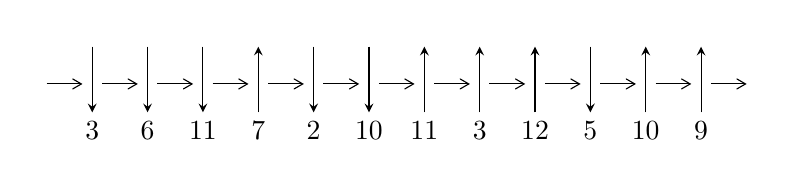
\begin{tikzpicture}[x=20pt, y=17pt]
	% nodes
	\node (C0) at (0, 0) {};
	\node (C1) at (1, 0) {};
	\node (C1U) at (1, +1) {};
	\node (C1D) at (1, -1) {3};

	\node (C2) at (2, 0) {};
	\node (C2U) at (2, +1) {};
	\node (C2D) at (2, -1) {6};

	\node (C3) at (3, 0) {};
	\node (C3U) at (3, +1) {};
	\node (C3D) at (3, -1) {11};

	\node (C4) at (4, 0) {};
	\node (C4U) at (4, +1) {};
	\node (C4D) at (4, -1) {7};

	\node (C5) at (5, 0) {};
	\node (C5U) at (5, +1) {};
	\node (C5D) at (5, -1) {2};

	\node (C6) at (6, 0) {};
	\node (C6U) at (6, +1) {};
	\node (C6D) at (6, -1) {10};

	\node (C7) at (7, 0) {};
	\node (C7U) at (7, +1) {};
	\node (C7D) at (7, -1) {11};

	\node (C8) at (8, 0) {};
	\node (C8U) at (8, +1) {};
	\node (C8D) at (8, -1) {3};

	\node (C9) at (9, 0) {};
	\node (C9U) at (9, +1) {};
	\node (C9D) at (9, -1) {12};

	\node (C10) at (10, 0) {};
	\node (C10U) at (10, +1) {};
	\node (C10D) at (10, -1) {5};

	\node (C11) at (11, 0) {};
	\node (C11U) at (11, +1) {};
	\node (C11D) at (11, -1) {10};

	\node (C12) at (12, 0) {};
	\node (C12U) at (12, +1) {};
	\node (C12D) at (12, -1) {9};
	\node (C13) at (13, 0) {};

	% arrows
	\draw[->,>={angle 60}]
	(C0) edge (C1) (C1) edge (C2) (C2) edge (C3) (C3) edge (C4) (C4) edge (C5) (C5) edge (C6) (C6) edge (C7) (C7) edge (C8) (C8) edge (C9) (C9) edge (C10) (C10) edge (C11) (C11) edge (C12) (C12) edge (C13) ;	\draw[->,>=stealth]
	(C1U) edge (C1D) (C2U) edge (C2D) (C3U) edge (C3D) (C4D) edge (C4U) (C5U) edge (C5D) (C6U) edge (C6D) (C7D) edge (C7U) (C8D) edge (C8U) (C9D) edge (C9U) (C10U) edge (C10D) (C11D) edge (C11U) (C12D) edge (C12U) ;
	\end{tikzpicture} \\
\hhline{~~} \\& 
\textbf{Solving Sequence} \\ \cline{2-2} 
 &
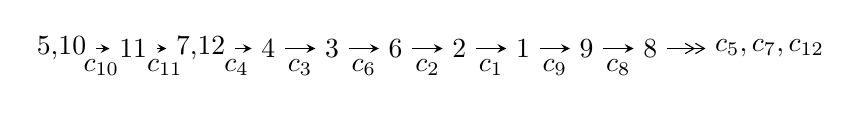
\begin{tikzpicture}[x=23pt, y=7pt]
	% node
	\node (A0) at (-1/8, 0) {5,10};
	\node (A1) at (1, 0) {11};
	\node (A2) at (33/16, 0) {7,12};
	\node (A3) at (25/8, 0) {4};
	\node (A4) at (33/8, 0) {3};
	\node (A5) at (41/8, 0) {6};
	\node (A6) at (49/8, 0) {2};
	\node (A7) at (57/8, 0) {1};
	\node (A8) at (65/8, 0) {9};
	\node (A9) at (73/8, 0) {8};
	\node (C1) at (1/2, -1) {$c_{10}$};
	\node (C2) at (3/2, -1) {$c_{11}$};
	\node (C3) at (21/8, -1) {$c_{4}$};
	\node (C4) at (29/8, -1) {$c_{3}$};
	\node (C5) at (37/8, -1) {$c_{6}$};
	\node (C6) at (45/8, -1) {$c_{2}$};
	\node (C7) at (53/8, -1) {$c_{1}$};
	\node (C8) at (61/8, -1) {$c_{9}$};
	\node (C9) at (69/8, -1) {$c_{8}$};
	\node (A10) at (11, 0) {$c_{5},c_{7},c_{12}$};

	% edge
	\draw[->,>=stealth]	
	(A0) edge (A1) (A1) edge (A2) (A2) edge (A3) (A3) edge (A4) (A4) edge (A5) (A5) edge (A6) (A6) edge (A7) (A7) edge (A8) (A8) edge (A9) ;
	\draw[->>,>={angle 60}]	
	(A9) edge (A10);
\end{tikzpicture} \\ 

\end{tabular} \\

\footnotetext{
The image of knot diagram is generated by the software ``\textbf{Draw programme}" developed by Andrew Bartholomew(\url{http://www.layer8.co.uk/maths/draw/index.htm\#Running-draw}), where we modified some parts for our purpose(\url{https://github.com/CATsTAILs/LinksPainter}).
}\phantom \\ \newline 
\centering \textbf{Ideals for irreducible components\footnotemark of $X_{\text{par}}$} 
 
\begin{align*}
I^u_{1}&=\langle 
-25033252 u^{22}+121557101 u^{21}+\cdots+292671322 b+456806862,\\
\phantom{I^u_{1}}&\phantom{= \langle  }157446473 u^{22}-71514300 u^{21}+\cdots+146335661 a-334256756,\;u^{23}- u^{22}+\cdots-4 u+1\rangle \\
I^u_{2}&=\langle 
- u^5 b+2 u^4 b- u^5- u^3 b+b^2-2 b u+2 b-2 u,\;- u^4+a-1,\;u^6+u^4+2 u^2+1\rangle \\
\\
\end{align*}
\raggedright * 2 irreducible components of $\dim_{\mathbb{C}}=0$, with total 35 representations.\\
\footnotetext{All coefficients of polynomials are rational numbers. But the coefficients are sometimes approximated in decimal forms when there is not enough margin.}
\newpage
\renewcommand{\arraystretch}{1}
\centering \section*{I. $I^u_{1}= \langle -2.50\times10^{7} u^{22}+1.22\times10^{8} u^{21}+\cdots+2.93\times10^{8} b+4.57\times10^{8},\;1.57\times10^{8} u^{22}-7.15\times10^{7} u^{21}+\cdots+1.46\times10^{8} a-3.34\times10^{8},\;u^{23}- u^{22}+\cdots-4 u+1 \rangle$}
\flushleft \textbf{(i) Arc colorings}\\
\begin{tabular}{m{7pt} m{180pt} m{7pt} m{180pt} }
\flushright $a_{5}=$&$\begin{pmatrix}0\\u\end{pmatrix}$ \\
\flushright $a_{10}=$&$\begin{pmatrix}1\\0\end{pmatrix}$ \\
\flushright $a_{11}=$&$\begin{pmatrix}1\\u^2\end{pmatrix}$ \\
\flushright $a_{7}=$&$\begin{pmatrix}-1.07593 u^{22}+0.488700 u^{21}+\cdots-6.60771 u+2.28418\\0.0855337 u^{22}-0.415337 u^{21}+\cdots+1.72095 u-1.56082\end{pmatrix}$ \\
\flushright $a_{12}=$&$\begin{pmatrix}u^2+1\\u^2\end{pmatrix}$ \\
\flushright $a_{4}=$&$\begin{pmatrix}-1.74252 u^{22}+1.41007 u^{21}+\cdots-7.48338 u+5.61498\\-0.341312 u^{22}-0.0869202 u^{21}+\cdots-0.317822 u+0.422860\end{pmatrix}$ \\
\flushright $a_{3}=$&$\begin{pmatrix}-2.02915 u^{22}+1.43160 u^{21}+\cdots-8.21390 u+5.70538\\-0.505038 u^{22}+0.0146154 u^{21}+\cdots-1.09158 u+0.687959\end{pmatrix}$ \\
\flushright $a_{6}=$&$\begin{pmatrix}-0.990393 u^{22}+0.0733639 u^{21}+\cdots-4.88676 u+0.723360\\0.0855337 u^{22}-0.415337 u^{21}+\cdots+1.72095 u-1.56082\end{pmatrix}$ \\
\flushright $a_{2}=$&$\begin{pmatrix}-0.0458208 u^{22}+0.256242 u^{21}+\cdots+1.37542 u+1.65212\\-0.626056 u^{22}+0.0915497 u^{21}+\cdots-1.35086 u+1.57783\end{pmatrix}$ \\
\flushright $a_{1}=$&$\begin{pmatrix}- u^6- u^4-2 u^2-1\\- u^6- u^2\end{pmatrix}$ \\
\flushright $a_{9}=$&$\begin{pmatrix}u^4+u^2+1\\u^4\end{pmatrix}$ \\
\flushright $a_{8}=$&$\begin{pmatrix}-0.580827 u^{22}-0.0431012 u^{21}+\cdots-3.61378 u+0.136133\\0.107132 u^{22}-0.226022 u^{21}+\cdots+1.07904 u-1.52412\end{pmatrix}$\\&\end{tabular}
\flushleft \textbf{(ii) Obstruction class $= -1$}\\~\\
\flushleft \textbf{(iii) Cusp Shapes $= \frac{670390078}{146335661} u^{22}-\frac{445304479}{146335661} u^{21}+\cdots+\frac{1755269129}{146335661} u-\frac{1610811133}{146335661}$}\\~\\
\newpage\renewcommand{\arraystretch}{1}
\flushleft \textbf{(iv) u-Polynomials at the component}\newline \\
\begin{tabular}{m{50pt}|m{274pt}}
Crossings & \hspace{64pt}u-Polynomials at each crossing \\
\hline $$\begin{aligned}c_{1}\end{aligned}$$&$\begin{aligned}
&u^{23}+19 u^{22}+\cdots-12 u+1
\end{aligned}$\\
\hline $$\begin{aligned}c_{2},c_{5}\end{aligned}$$&$\begin{aligned}
&u^{23}+u^{22}+\cdots+6 u+1
\end{aligned}$\\
\hline $$\begin{aligned}c_{3}\end{aligned}$$&$\begin{aligned}
&u^{23}+5 u^{22}+\cdots+138708 u+29957
\end{aligned}$\\
\hline $$\begin{aligned}c_{4},c_{8}\end{aligned}$$&$\begin{aligned}
&u^{23}+u^{22}+\cdots-140 u+25
\end{aligned}$\\
\hline $$\begin{aligned}c_{6}\end{aligned}$$&$\begin{aligned}
&u^{23}+7 u^{22}+\cdots-11462 u-5383
\end{aligned}$\\
\hline $$\begin{aligned}c_{7}\end{aligned}$$&$\begin{aligned}
&u^{23}+u^{22}+\cdots+376 u-7
\end{aligned}$\\
\hline $$\begin{aligned}c_{9},c_{11},c_{12}\end{aligned}$$&$\begin{aligned}
&u^{23}-3 u^{22}+\cdots+6 u+1
\end{aligned}$\\
\hline $$\begin{aligned}c_{10}\end{aligned}$$&$\begin{aligned}
&u^{23}- u^{22}+\cdots-4 u+1
\end{aligned}$\\
\hline
\end{tabular}\\~\\
\newpage\renewcommand{\arraystretch}{1}
\flushleft \textbf{(v) Riley Polynomials at the component}\newline \\
\begin{tabular}{m{50pt}|m{274pt}}
Crossings & \hspace{64pt}Riley Polynomials at each crossing \\
\hline $$\begin{aligned}c_{1}\end{aligned}$$&$\begin{aligned}
&y^{23}-23 y^{22}+\cdots-984 y-1
\end{aligned}$\\
\hline $$\begin{aligned}c_{2},c_{5}\end{aligned}$$&$\begin{aligned}
&y^{23}-19 y^{22}+\cdots-12 y-1
\end{aligned}$\\
\hline $$\begin{aligned}c_{3}\end{aligned}$$&$\begin{aligned}
&y^{23}-73 y^{22}+\cdots-10832245444 y-897421849
\end{aligned}$\\
\hline $$\begin{aligned}c_{4},c_{8}\end{aligned}$$&$\begin{aligned}
&y^{23}+43 y^{22}+\cdots+8150 y-625
\end{aligned}$\\
\hline $$\begin{aligned}c_{6}\end{aligned}$$&$\begin{aligned}
&y^{23}-41 y^{22}+\cdots+193389604 y-28976689
\end{aligned}$\\
\hline $$\begin{aligned}c_{7}\end{aligned}$$&$\begin{aligned}
&y^{23}+43 y^{22}+\cdots+163692 y-49
\end{aligned}$\\
\hline $$\begin{aligned}c_{9},c_{11},c_{12}\end{aligned}$$&$\begin{aligned}
&y^{23}+39 y^{22}+\cdots+30 y-1
\end{aligned}$\\
\hline $$\begin{aligned}c_{10}\end{aligned}$$&$\begin{aligned}
&y^{23}+3 y^{22}+\cdots+6 y-1
\end{aligned}$\\
\hline
\end{tabular}\\~\\
\newpage\flushleft \textbf{(vi) Complex Volumes and Cusp Shapes}
$$\begin{array}{c|c|c}  
\text{Solutions to }I^u_{1}& \I (\text{vol} + \sqrt{-1}CS) & \text{Cusp shape}\\
 \hline 
\begin{aligned}
u &= \phantom{-}0.638291 + 0.756340 I \\
a &= -0.053920 + 0.672113 I \\
b &= -1.27006 - 0.66289 I\end{aligned}
 & -2.28180 - 5.04874 I & -2.29238 + 7.64932 I \\ \hline\begin{aligned}
u &= \phantom{-}0.638291 - 0.756340 I \\
a &= -0.053920 - 0.672113 I \\
b &= -1.27006 + 0.66289 I\end{aligned}
 & -2.28180 + 5.04874 I & -2.29238 - 7.64932 I \\ \hline\begin{aligned}
u &= \phantom{-}0.728457 + 0.859772 I \\
a &= -0.696631 - 0.653322 I \\
b &= \phantom{-}0.729953 + 0.669715 I\end{aligned}
 & -4.64426 - 2.76660 I & -5.38126 + 3.37592 I \\ \hline\begin{aligned}
u &= \phantom{-}0.728457 - 0.859772 I \\
a &= -0.696631 + 0.653322 I \\
b &= \phantom{-}0.729953 - 0.669715 I\end{aligned}
 & -4.64426 + 2.76660 I & -5.38126 - 3.37592 I \\ \hline\begin{aligned}
u &= \phantom{-}0.356533 + 0.788524 I \\
a &= \phantom{-}1.151030 + 0.050949 I \\
b &= -1.04769 + 1.09696 I\end{aligned}
 & -1.92628 + 1.02137 I & -4.36487 - 0.00463 I \\ \hline\begin{aligned}
u &= \phantom{-}0.356533 - 0.788524 I \\
a &= \phantom{-}1.151030 - 0.050949 I \\
b &= -1.04769 - 1.09696 I\end{aligned}
 & -1.92628 - 1.02137 I & -4.36487 + 0.00463 I \\ \hline\begin{aligned}
u &= -0.087548 + 0.829182 I \\
a &= -0.165345 - 0.286028 I \\
b &= \phantom{-}1.012130 + 0.803767 I\end{aligned}
 & \phantom{-}1.16140 + 1.81818 I & \phantom{-}6.31882 - 4.29104 I \\ \hline\begin{aligned}
u &= -0.087548 - 0.829182 I \\
a &= -0.165345 + 0.286028 I \\
b &= \phantom{-}1.012130 - 0.803767 I\end{aligned}
 & \phantom{-}1.16140 - 1.81818 I & \phantom{-}6.31882 + 4.29104 I \\ \hline\begin{aligned}
u &= -0.370099 + 0.602173 I \\
a &= \phantom{-}0.256458 - 0.802239 I \\
b &= -0.536912 + 0.631160 I\end{aligned}
 & \phantom{-}0.076790 + 1.263270 I & \phantom{-}0.68970 - 5.37175 I \\ \hline\begin{aligned}
u &= -0.370099 - 0.602173 I \\
a &= \phantom{-}0.256458 + 0.802239 I \\
b &= -0.536912 - 0.631160 I\end{aligned}
 & \phantom{-}0.076790 - 1.263270 I & \phantom{-}0.68970 + 5.37175 I\\
 \hline 
 \end{array}$$\newpage$$\begin{array}{c|c|c}  
\text{Solutions to }I^u_{1}& \I (\text{vol} + \sqrt{-1}CS) & \text{Cusp shape}\\
 \hline 
\begin{aligned}
u &= -1.076080 + 0.763334 I \\
a &= -0.18671 + 1.49317 I \\
b &= \phantom{-}1.74353 - 0.51727 I\end{aligned}
 & -11.04540 + 2.65995 I & -6.14199 - 2.02854 I \\ \hline\begin{aligned}
u &= -1.076080 - 0.763334 I \\
a &= -0.18671 - 1.49317 I \\
b &= \phantom{-}1.74353 + 0.51727 I\end{aligned}
 & -11.04540 - 2.65995 I & -6.14199 + 2.02854 I \\ \hline\begin{aligned}
u &= -0.674267\phantom{ +0.000000I} \\
a &= \phantom{-}1.27270\phantom{ +0.000000I} \\
b &= \phantom{-}0.595901\phantom{ +0.000000I}\end{aligned}
 & -1.85226\phantom{ +0.000000I} & -5.67690\phantom{ +0.000000I} \\ \hline\begin{aligned}
u &= -0.767551 + 1.147080 I \\
a &= -1.301880 + 0.405799 I \\
b &= \phantom{-}2.41969 + 0.70458 I\end{aligned}
 & -9.61269 + 4.18878 I & -5.20065 - 2.68941 I \\ \hline\begin{aligned}
u &= -0.767551 - 1.147080 I \\
a &= -1.301880 - 0.405799 I \\
b &= \phantom{-}2.41969 - 0.70458 I\end{aligned}
 & -9.61269 - 4.18878 I & -5.20065 + 2.68941 I \\ \hline\begin{aligned}
u &= -1.01450 + 1.01430 I \\
a &= \phantom{-}1.01669 - 1.12066 I \\
b &= -1.98063 + 0.31926 I\end{aligned}
 & -18.6458 + 3.7213 I & -3.19708 - 1.97285 I \\ \hline\begin{aligned}
u &= -1.01450 - 1.01430 I \\
a &= \phantom{-}1.01669 + 1.12066 I \\
b &= -1.98063 - 0.31926 I\end{aligned}
 & -18.6458 - 3.7213 I & -3.19708 + 1.97285 I \\ \hline\begin{aligned}
u &= \phantom{-}1.10481 + 0.91677 I \\
a &= \phantom{-}1.22917 + 1.03499 I \\
b &= -1.37206 + 0.92349 I\end{aligned}
 & \phantom{-}15.8685 + 3.3875 I & -5.25744 - 0.65270 I \\ \hline\begin{aligned}
u &= \phantom{-}1.10481 - 0.91677 I \\
a &= \phantom{-}1.22917 - 1.03499 I \\
b &= -1.37206 - 0.92349 I\end{aligned}
 & \phantom{-}15.8685 - 3.3875 I & -5.25744 + 0.65270 I \\ \hline\begin{aligned}
u &= \phantom{-}0.94898 + 1.10084 I \\
a &= \phantom{-}0.84505 + 1.21860 I \\
b &= -2.63899 - 1.28859 I\end{aligned}
 & \phantom{-}16.5464 - 10.8721 I & -4.62089 + 4.80987 I\\
 \hline 
 \end{array}$$\newpage$$\begin{array}{c|c|c}  
\text{Solutions to }I^u_{1}& \I (\text{vol} + \sqrt{-1}CS) & \text{Cusp shape}\\
 \hline 
\begin{aligned}
u &= \phantom{-}0.94898 - 1.10084 I \\
a &= \phantom{-}0.84505 - 1.21860 I \\
b &= -2.63899 + 1.28859 I\end{aligned}
 & \phantom{-}16.5464 + 10.8721 I & -4.62089 - 4.80987 I \\ \hline\begin{aligned}
u &= \phantom{-}0.375835 + 0.114241 I \\
a &= -1.23027 - 2.62777 I \\
b &= -0.856913 + 0.343009 I\end{aligned}
 & -1.84255 - 2.10614 I & -6.71348 + 2.97651 I \\ \hline\begin{aligned}
u &= \phantom{-}0.375835 - 0.114241 I \\
a &= -1.23027 + 2.62777 I \\
b &= -0.856913 - 0.343009 I\end{aligned}
 & -1.84255 + 2.10614 I & -6.71348 - 2.97651 I\\
 \hline 
 \end{array}$$\newpage\newpage\renewcommand{\arraystretch}{1}
\centering \section*{II. $I^u_{2}= \langle - u^5 b- u^5+\cdots+b^2+2 b,\;- u^4+a-1,\;u^6+u^4+2 u^2+1 \rangle$}
\flushleft \textbf{(i) Arc colorings}\\
\begin{tabular}{m{7pt} m{180pt} m{7pt} m{180pt} }
\flushright $a_{5}=$&$\begin{pmatrix}0\\u\end{pmatrix}$ \\
\flushright $a_{10}=$&$\begin{pmatrix}1\\0\end{pmatrix}$ \\
\flushright $a_{11}=$&$\begin{pmatrix}1\\u^2\end{pmatrix}$ \\
\flushright $a_{7}=$&$\begin{pmatrix}u^4+1\\b\end{pmatrix}$ \\
\flushright $a_{12}=$&$\begin{pmatrix}u^2+1\\u^2\end{pmatrix}$ \\
\flushright $a_{4}=$&$\begin{pmatrix}- u^5- u^3-2 u\\- u^5 b- b u+u\end{pmatrix}$ \\
\flushright $a_{3}=$&$\begin{pmatrix}- u^5 b- u^5- u^3- b u-2 u\\u^3 b+u\end{pmatrix}$ \\
\flushright $a_{6}=$&$\begin{pmatrix}u^4+b+1\\b\end{pmatrix}$ \\
\flushright $a_{2}=$&$\begin{pmatrix}- u^5 b- u^5- u^4- u^3- b u-2 u-1\\- u^5+u^3 b- u^3+b- u\end{pmatrix}$ \\
\flushright $a_{1}=$&$\begin{pmatrix}0\\- u^4- u^2-1\end{pmatrix}$ \\
\flushright $a_{9}=$&$\begin{pmatrix}u^4+u^2+1\\u^4\end{pmatrix}$ \\
\flushright $a_{8}=$&$\begin{pmatrix}2 u^4+u^2+b+2\\u^2 b- u^2+b-1\end{pmatrix}$\\&\end{tabular}
\flushleft \textbf{(ii) Obstruction class $= 1$}\\~\\
\flushleft \textbf{(iii) Cusp Shapes $= -4 u^5+4 u^4-4 b u+4 u^2-4 u$}\\~\\
\newpage\renewcommand{\arraystretch}{1}
\flushleft \textbf{(iv) u-Polynomials at the component}\newline \\
\begin{tabular}{m{50pt}|m{274pt}}
Crossings & \hspace{64pt}u-Polynomials at each crossing \\
\hline $$\begin{aligned}c_{1}\end{aligned}$$&$\begin{aligned}
&(u^2- u+1)^6
\end{aligned}$\\
\hline $$\begin{aligned}c_{2},c_{5}\end{aligned}$$&$\begin{aligned}
&(u^4- u^2+1)^3
\end{aligned}$\\
\hline $$\begin{aligned}c_{3}\end{aligned}$$&$\begin{aligned}
&u^{12}+6 u^{10}+\cdots-4 u+1
\end{aligned}$\\
\hline $$\begin{aligned}c_{4},c_{8}\end{aligned}$$&$\begin{aligned}
&(u^2+1)^6
\end{aligned}$\\
\hline $$\begin{aligned}c_{6}\end{aligned}$$&$\begin{aligned}
&u^{12}-6 u^{10}+\cdots+2 u+1
\end{aligned}$\\
\hline $$\begin{aligned}c_{7}\end{aligned}$$&$\begin{aligned}
&u^{12}-4 u^{11}+\cdots-70 u+37
\end{aligned}$\\
\hline $$\begin{aligned}c_{9}\end{aligned}$$&$\begin{aligned}
&(u^3+u^2+2 u+1)^4
\end{aligned}$\\
\hline $$\begin{aligned}c_{10}\end{aligned}$$&$\begin{aligned}
&(u^6+u^4+2 u^2+1)^2
\end{aligned}$\\
\hline $$\begin{aligned}c_{11},c_{12}\end{aligned}$$&$\begin{aligned}
&(u^3- u^2+2 u-1)^4
\end{aligned}$\\
\hline
\end{tabular}\\~\\
\newpage\renewcommand{\arraystretch}{1}
\flushleft \textbf{(v) Riley Polynomials at the component}\newline \\
\begin{tabular}{m{50pt}|m{274pt}}
Crossings & \hspace{64pt}Riley Polynomials at each crossing \\
\hline $$\begin{aligned}c_{1}\end{aligned}$$&$\begin{aligned}
&(y^2+y+1)^6
\end{aligned}$\\
\hline $$\begin{aligned}c_{2},c_{5}\end{aligned}$$&$\begin{aligned}
&(y^2- y+1)^6
\end{aligned}$\\
\hline $$\begin{aligned}c_{3}\end{aligned}$$&$\begin{aligned}
&y^{12}+12 y^{11}+\cdots-6 y+1
\end{aligned}$\\
\hline $$\begin{aligned}c_{4},c_{8}\end{aligned}$$&$\begin{aligned}
&(y+1)^{12}
\end{aligned}$\\
\hline $$\begin{aligned}c_{6}\end{aligned}$$&$\begin{aligned}
&y^{12}-12 y^{11}+\cdots+6 y+1
\end{aligned}$\\
\hline $$\begin{aligned}c_{7}\end{aligned}$$&$\begin{aligned}
&y^{12}+8 y^{11}+\cdots+1094 y+1369
\end{aligned}$\\
\hline $$\begin{aligned}c_{9},c_{11},c_{12}\end{aligned}$$&$\begin{aligned}
&(y^3+3 y^2+2 y-1)^4
\end{aligned}$\\
\hline $$\begin{aligned}c_{10}\end{aligned}$$&$\begin{aligned}
&(y^3+y^2+2 y+1)^4
\end{aligned}$\\
\hline
\end{tabular}\\~\\
\newpage\flushleft \textbf{(vi) Complex Volumes and Cusp Shapes}
$$\begin{array}{c|c|c}  
\text{Solutions to }I^u_{2}& \I (\text{vol} + \sqrt{-1}CS) & \text{Cusp shape}\\
 \hline 
\begin{aligned}
u &= \phantom{-}0.744862 + 0.877439 I \\
a &= -0.662359 - 0.562280 I \\
b &= -0.192400 + 0.406511 I\end{aligned}
 & -4.66906 - 4.85801 I & -5.50976 + 6.44355 I \\ \hline\begin{aligned}
u &= \phantom{-}0.744862 + 0.877439 I \\
a &= -0.662359 - 0.562280 I \\
b &= \phantom{-}0.95484 + 1.38041 I\end{aligned}
 & -4.66906 - 0.79824 I & -5.50976 - 0.48465 I \\ \hline\begin{aligned}
u &= \phantom{-}0.744862 - 0.877439 I \\
a &= -0.662359 + 0.562280 I \\
b &= -0.192400 - 0.406511 I\end{aligned}
 & -4.66906 + 4.85801 I & -5.50976 - 6.44355 I \\ \hline\begin{aligned}
u &= \phantom{-}0.744862 - 0.877439 I \\
a &= -0.662359 + 0.562280 I \\
b &= \phantom{-}0.95484 - 1.38041 I\end{aligned}
 & -4.66906 + 0.79824 I & -5.50976 + 0.48465 I \\ \hline\begin{aligned}
u &= -0.744862 + 0.877439 I \\
a &= -0.662359 + 0.562280 I \\
b &= \phantom{-}0.369879 + 0.255848 I\end{aligned}
 & -4.66906 + 0.79824 I & -5.50976 + 0.48465 I \\ \hline\begin{aligned}
u &= -0.744862 + 0.877439 I \\
a &= -0.662359 + 0.562280 I \\
b &= \phantom{-}1.51712 - 0.71805 I\end{aligned}
 & -4.66906 + 4.85801 I & -5.50976 - 6.44355 I \\ \hline\begin{aligned}
u &= -0.744862 - 0.877439 I \\
a &= -0.662359 - 0.562280 I \\
b &= \phantom{-}0.369879 - 0.255848 I\end{aligned}
 & -4.66906 - 0.79824 I & -5.50976 - 0.48465 I \\ \hline\begin{aligned}
u &= -0.744862 - 0.877439 I \\
a &= -0.662359 - 0.562280 I \\
b &= \phantom{-}1.51712 + 0.71805 I\end{aligned}
 & -4.66906 - 4.85801 I & -5.50976 + 6.44355 I \\ \hline\begin{aligned}
u &= \phantom{-0.000000 -}0.754878 I \\
a &= \phantom{-}1.32472\phantom{ +0.000000I} \\
b &= -0.177479 + 0.662359 I\end{aligned}
 & -0.53148 + 2.02988 I & \phantom{-}1.01951 - 3.46410 I \\ \hline\begin{aligned}
u &= \phantom{-0.000000 -}0.754878 I \\
a &= \phantom{-}1.32472\phantom{ +0.000000I} \\
b &= -2.47196 + 0.66236 I\end{aligned}
 & -0.53148 - 2.02988 I & \phantom{-}1.01951 + 3.46410 I\\
 \hline 
 \end{array}$$\newpage$$\begin{array}{c|c|c}  
\text{Solutions to }I^u_{2}& \I (\text{vol} + \sqrt{-1}CS) & \text{Cusp shape}\\
 \hline 
\begin{aligned}
u &= \phantom{-0.000000 } -0.754878 I \\
a &= \phantom{-}1.32472\phantom{ +0.000000I} \\
b &= -0.177479 - 0.662359 I\end{aligned}
 & -0.53148 - 2.02988 I & \phantom{-}1.01951 + 3.46410 I \\ \hline\begin{aligned}
u &= \phantom{-0.000000 } -0.754878 I \\
a &= \phantom{-}1.32472\phantom{ +0.000000I} \\
b &= -2.47196 - 0.66236 I\end{aligned}
 & -0.53148 + 2.02988 I & \phantom{-}1.01951 - 3.46410 I\\
 \hline 
 \end{array}$$\newpage
\newpage\renewcommand{\arraystretch}{1}
\centering \section*{ III. u-Polynomials}
\begin{tabular}{m{50pt}|m{274pt}}
Crossings & \hspace{64pt}u-Polynomials at each crossing \\
\hline $$\begin{aligned}c_{1}\end{aligned}$$&$\begin{aligned}
&((u^2- u+1)^6)(u^{23}+19 u^{22}+\cdots-12 u+1)
\end{aligned}$\\
\hline $$\begin{aligned}c_{2},c_{5}\end{aligned}$$&$\begin{aligned}
&((u^4- u^2+1)^3)(u^{23}+u^{22}+\cdots+6 u+1)
\end{aligned}$\\
\hline $$\begin{aligned}c_{3}\end{aligned}$$&$\begin{aligned}
&(u^{12}+6 u^{10}+\cdots-4 u+1)(u^{23}+5 u^{22}+\cdots+138708 u+29957)
\end{aligned}$\\
\hline $$\begin{aligned}c_{4},c_{8}\end{aligned}$$&$\begin{aligned}
&((u^2+1)^6)(u^{23}+u^{22}+\cdots-140 u+25)
\end{aligned}$\\
\hline $$\begin{aligned}c_{6}\end{aligned}$$&$\begin{aligned}
&(u^{12}-6 u^{10}+\cdots+2 u+1)(u^{23}+7 u^{22}+\cdots-11462 u-5383)
\end{aligned}$\\
\hline $$\begin{aligned}c_{7}\end{aligned}$$&$\begin{aligned}
&(u^{12}-4 u^{11}+\cdots-70 u+37)(u^{23}+u^{22}+\cdots+376 u-7)
\end{aligned}$\\
\hline $$\begin{aligned}c_{9}\end{aligned}$$&$\begin{aligned}
&((u^3+u^2+2 u+1)^4)(u^{23}-3 u^{22}+\cdots+6 u+1)
\end{aligned}$\\
\hline $$\begin{aligned}c_{10}\end{aligned}$$&$\begin{aligned}
&((u^6+u^4+2 u^2+1)^2)(u^{23}- u^{22}+\cdots-4 u+1)
\end{aligned}$\\
\hline $$\begin{aligned}c_{11},c_{12}\end{aligned}$$&$\begin{aligned}
&((u^3- u^2+2 u-1)^4)(u^{23}-3 u^{22}+\cdots+6 u+1)
\end{aligned}$\\
\hline
\end{tabular}\newpage\renewcommand{\arraystretch}{1}
\centering \section*{ IV. Riley Polynomials}
\begin{tabular}{m{50pt}|m{274pt}}
Crossings & \hspace{64pt}Riley Polynomials at each crossing \\
\hline $$\begin{aligned}c_{1}\end{aligned}$$&$\begin{aligned}
&((y^2+y+1)^6)(y^{23}-23 y^{22}+\cdots-984 y-1)
\end{aligned}$\\
\hline $$\begin{aligned}c_{2},c_{5}\end{aligned}$$&$\begin{aligned}
&((y^2- y+1)^6)(y^{23}-19 y^{22}+\cdots-12 y-1)
\end{aligned}$\\
\hline $$\begin{aligned}c_{3}\end{aligned}$$&$\begin{aligned}
&(y^{12}+12 y^{11}+\cdots-6 y+1)\\
&\cdot(y^{23}-73 y^{22}+\cdots-10832245444 y-897421849)
\end{aligned}$\\
\hline $$\begin{aligned}c_{4},c_{8}\end{aligned}$$&$\begin{aligned}
&((y+1)^{12})(y^{23}+43 y^{22}+\cdots+8150 y-625)
\end{aligned}$\\
\hline $$\begin{aligned}c_{6}\end{aligned}$$&$\begin{aligned}
&(y^{12}-12 y^{11}+\cdots+6 y+1)\\
&\cdot(y^{23}-41 y^{22}+\cdots+193389604 y-28976689)
\end{aligned}$\\
\hline $$\begin{aligned}c_{7}\end{aligned}$$&$\begin{aligned}
&(y^{12}+8 y^{11}+\cdots+1094 y+1369)(y^{23}+43 y^{22}+\cdots+163692 y-49)
\end{aligned}$\\
\hline $$\begin{aligned}c_{9},c_{11},c_{12}\end{aligned}$$&$\begin{aligned}
&((y^3+3 y^2+2 y-1)^4)(y^{23}+39 y^{22}+\cdots+30 y-1)
\end{aligned}$\\
\hline $$\begin{aligned}c_{10}\end{aligned}$$&$\begin{aligned}
&((y^3+y^2+2 y+1)^4)(y^{23}+3 y^{22}+\cdots+6 y-1)
\end{aligned}$\\
\hline
\end{tabular}
\vskip 2pc
\end{document}